\documentclass{sbc2019}%

\usepackage{graphicx,url}
\usepackage[utf8]{inputenc}
\usepackage[misc,geometry]{ifsym} 
\usepackage{fontspec}
\usepackage{fontawesome}
\usepackage{academicons}
\usepackage{color}
\usepackage{hyperref} 
\usepackage{aas_macros}
\usepackage[bottom]{footmisc}
\usepackage{supertabular}
\usepackage{afterpage}
\usepackage{url}
\usepackage{pifont}
\usepackage{multicol}
\usepackage{multirow}
\usepackage{amssymb}
\usepackage{syntax}

\setcitestyle{square}

\definecolor{orcidlogo}{rgb}{0.37,0.48,0.13}
\definecolor{unilogo}{rgb}{0.16, 0.26, 0.58}
\definecolor{maillogo}{rgb}{0.58, 0.16, 0.26}
\definecolor{darkblue}{rgb}{0.0,0.0,0.0}
\hypersetup{colorlinks,breaklinks,
            linkcolor=darkblue,urlcolor=darkblue,
            anchorcolor=darkblue,citecolor=darkblue}
%\hypersetup{colorlinks,citecolor=blue,linkcolor=blue,urlcolor=blue}

%%%%%%% IMPORTANT: We disable hyperlinks by default with this line, to avoid the error "\pdfendlink ended up in different nesting level" while writing.
%\hypersetup{draft}

%\jid{JBCS}
\jid{JIDM}
\jtitle{Journal of Information and Data Management, 2024, 13:1, }
\doi{10.5753/jidm.2024.XXXXXX}
\copyrightstatement{This work is licensed under a Creative Commons Attribution 4.0 International License}
\jyear{2023}


\newtheorem{example}{Example}
\newtheorem{definition}{Definition}

\title{JFUSE: Json FUll Schema Extractor}

\author[Banhara et at. 2025]{
 \affil{Natália Banhara~\textcolor{blue}{\faEnvelopeO}~~[~\textbf{Universidade Federal da Fronteira Sul}~|\href{mailto:natalia.banhara@outlook.com}{~\textbf{\textit{natalia.banhara@outlook.com}}}~]} 
  \affil{Geomar A. Schreiner~[~\textbf{Universidade Federal da Fronteira Sul}~|{~\textbf{\textit{gschreiner@uffs.edu.br}}}~]} 
  \affil{Samuel da Silva Feitosa~[~\textbf{Universidade Federal da Fronteira Sul}~|{~\textbf{\textit{samuel.feitosa@uffs.edu.br}}}~]} 
  \affil{Denio Duarte~[~\textbf{Universidade Federal da Fronteira Sul}~|{~\textbf{\textit{duarte@uffs.edu.br}}}~]}
}


\begin{document} 

\begin{frontmatter}

\maketitle

\begin{mail}
Universidade Federal da Fronteira Sul, Rodovia SC 484 - Km 02, Fronteira Sul, CEP 89815-899, Chapecó, SC, Brazil.
\end{mail}

\begin{dates}
\small{\textbf{Received:} DD Month YYYY~~~$\bullet$~~~\textbf{Accepted:} DD Month YYYY~~~$\bullet$~~~\textbf{Published:} DD Month YYYY}
%Full list of authors' information is available at the end of the article.
\end{dates}

\begin{abstract}
Recently, JSON became a trendy data format for representing datasets. 
Its success is due to embodying structure and data in the same representation. 
Moreover, it has a loose structure, i.e., the structure (aka schema) is not rigid. 
While the absence of a rigid schema brings several advantages, it is impossible to exploit some benefits of knowing the schema in advance, such as query and storage optimization and improving data curation. 
In this paper, we propose JFUSE, a tool to deal with the problem of discovering a schema from JSON collections. Besides inferring basic types (e.g., atomic types, arrays, and objects), JFUSE also discovers enumeration, tagged unions, metadata as data, objects as collections, and arrays as tuples. 
We propose a metamodel that can be easily transformed into any schema language (e.g., JSON Schema). 
Our experiments show that the proposed approach infers concise and correct schemas from (huge) JSON collections.
\end{abstract}
     
\begin{keywords}
Schema Discovering, JSON, Metamodel
\end{keywords}

\end{frontmatter}

\section{Introduction}
\label{sec:intro}

\color{blue} 

Lately, we witness a flood of data generated by several data-centric applications. 
Some areas of science, for example, are facing a huge increase of data volumes from satellites, telescopes, high-throughput instruments, sensor networks, accelerators, and supercomputers~\citep{BHS09}. 
The generated data are mostly weakly structured, irregular, and incomplete~\citep{Ke+22}; besides they do not follow a predefined schema. 
To store and exchange this kind of data, JSON has become one of the most popular formats~\citep{bourhis2017json}. 
JSON is a lightweight format and its documents are collections of key-value pairs, i.e., it stores data (value) and metadata (key) altogether a given document. 
This structure makes JSON documents be loosely coupled with schemas. 
On the other hand, applications that need to access this kind of data must have some reliable notion of its schema. 

Schemas are essential for data-centric applications, and \citep{Ke+22} show some tasks which schemas can be usuful:

\begin{itemize}

  \item Source Selection: it allows to choose the best data source for what users are looking for,
   
  \item Query Formulation: schemas decribe the content of a data source and so give a better overview of the content to be queried. 
  This is also true when a query must be decopomsed or optimized. 
  Knowing the documents structures makes easier to query multiple datas ource to find the best query decomposition.

  \item Data Indexing: the schema of a data source $\mathcal{D}$ may be a guide to built indexes on $\mathcal{D}$.
  
  \item Query Answering: the schema of a data source $\mathcal{D}$ allows to detemine whether or not a subset of $\mathcal{D}$ contains the answer of a given query.
  
  \item Data integration: the use of schema information to combine data sources is essential to achieve better results.
  
  \item Data Quality Assessment: schemas allow to use metrics to evaluate the quality of a data source, e.g., the completeness of a dataset reagarding its schema.
  
  \item Data Partitioning: when data must be distribute in multiple nodes, schema enable a better partioning plan.
\end{itemize} 

\color{black} 

Given a collection of JSON documents, extracting the latent schema presents a challenge due to its inherently flexible and dynamic nature ~\citep{canovas2013discovering}. JSON allows nested objects, arrays, and various structures with no enforced schema, making it difficult to infer a consistent and accurate schema. 
These complexities and the advantages of using a schema create a necessity for schema extraction approaches. 

Many schema extraction approaches have been proposed based on the importance of a schema ~\citep{frozza2018approach, baazizi2019parametric,abdelhedi2021automatic, klessinger2022extracting}. Each one explores the schema extraction on different faces of the JSON with distinct approaches. All approaches extract the basic JSON types (string, number, boolean, object, and array) but differ on the other JSON features (\textit{e.g.} tagged union, and enumerations). The works of Frozza et al. (2018), Baazizi et al. (2019), and Abdelhedi et al. (2021) focus only on the extraction of the basic types. Namba and Mior (2021), and Spoth et al. (2021) propose complete tools; however, they cannot discover tagged unions and enumerations. Although Klessinger et al. (2022) include tagged unions in the target schema, other types are not considered. 
Despite schema extraction being addressed in the state of the art, we are unaware of any approach that deals with the JSON structure complexity. 

In this paper, we present \textit{JFUSE} (Json FUll Schema Extractor), a novel approach for schema extraction. Our approach maps the JSON fields to vertices and uses edges to map relationships between them (\textit{e.g.}, parenting or sibling). In the graph, we store information about the occurrence of each field and their relationship to facilitate the inference of the schema. Based on the graph, we generate a metamodel representing the schema rules. Our approach can extract information about the basic JSON data types and features like tagged unions, enumeration, data collections, and tuples encoded in arrays.
\color{blue} 
It extends the work presented in \cite{Ba+24}. 
The new contributions are as follows: ($i$) keys constraints are now extracted, ($ii$) new experiments are conducted, and ($iii$)


\color{black}

We validate JFUSE executing two sets of experiments. The first one is to validate the approach against real-world datasets, evaluating the quality of the extracted schema. The second experiment focuses on proving the approach's concept, testing the extraction against a synthetic dataset created based on the different facets of a JSON (basic types, tagged union, tuple, array, metadata, object collection, and enumeration). The results show a concise schema regarding the size of the input collections and a satisfactory execution time. Moreover, the experiments also showed that our approach is scalable. 


The rest of this paper is organized as follows: Section \ref{sec:prelim} reviews the JSON data model and the main schema concepts. Section \ref{sec:RW} presents the related work, highlighting the limitations of the existing approaches. Section ~\ref{sec:SchDisc} details our graph-based methodology, including the definitions of the meta-model. Section ~\ref{sec:ResDisc}  presents the experimental results and discussion. Finally, Section ~\ref{sec:Concl} concludes the paper.


%\section{Preliminaries}
%  \label{sec:prelim}

\section{JSON and JSON Schema}
  \label{sec:prelim}

JSON (JavaScript Object Notation) is a lightweight data interchange format commonly used in modern web development and transmission protocols~\citep{bourhis2017json, Pezoa16, peng2011using}. 
A JSON is an unordered set of \textit{key-value} pairs~\citep{peng2011using}. Keys are strings; the values are weakly typed and may be primitive or complex~\citep{baazizi2019parametric}. Figure~\ref{fig:JSONEx} shows a JSON example.

A primitive JSON type is a Boolean ($\mathbb{B}$), a number ($\mathbb{R}$), a string ($\mathbb{S}$), or a \textit{NULL} value~\citep{bourhis2017json}. In Figure~\ref{fig:JSONEx}, the key \textit{type} (line 3) has an  $\mathbb{S}$ (string) value (\textit{`cinematography'}), another example, is the key \textit{year}, which  holds a $\mathbb{R}$ value. 


\begin{figure*}[ht]
    \centering
    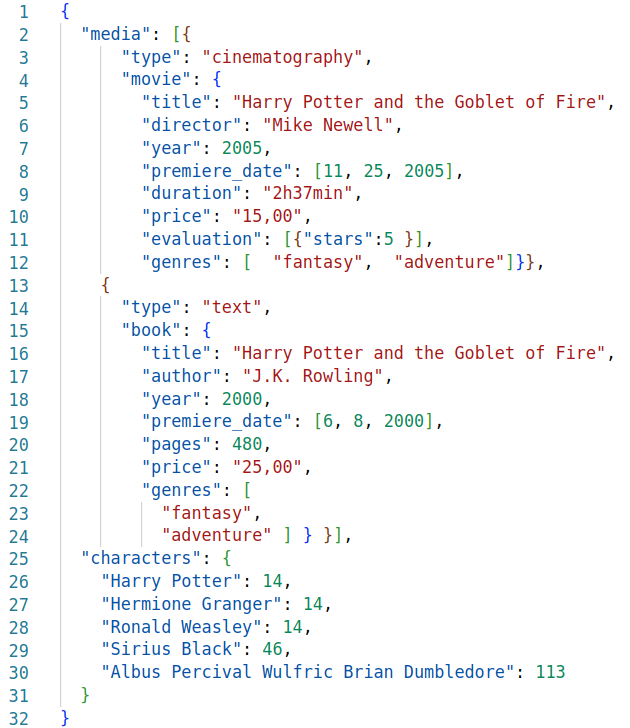
\includegraphics[scale=.45]{Figures/JSONExampleNew.png}
    \caption{An extract of JSON collection: running example}
    \label{fig:JSONEx}
\end{figure*}



A JSON value can also be from a complex type. A complex value type is either an object or an array. A JSON array $\mathcal{A}=[\tau_0, \tau_1,\ldots,\tau_N]$ is a sequence of \textit{N} JSON values (primitive or complex)~\citep{Sp+21}. In Figure~\ref{fig:JSONEx}, the key \textit{media} (line $2$) is an array of complex elements, and the keys \textit{premiere\_date} (lines $8$ and $19$) and \textit{genres} (lines $12$ and $22$) are arrays of primitive elements (\textit{i.e.}, $\mathbb{R}$ and $\mathbb{S}$).

In schema extraction, arrays are extracted as data collections~\citep{Sp+21} since they are a sequence of values. However, in some cases, an array can represent an encoded tuple. 
In the example, the key  \textit{premiere\_date} has three $\mathbb{R}$ values in each occurrence representing a date (month, day, and year) encoded in an array. A naive schema extraction approach will define the field as an ordinary array, losing information about its structure~\citep{Sp+21}.


The last complex type of JSON value is an object. A JSON object $\mathcal{O} = \{ k_1:\tau_1,\ldots,k_N:\tau_N\}$ is a set of keys $k_1...k_N$ mapped to values $\tau_1,\ldots,\tau_N$ of JSON types (primitive or complex)~\citep{Sp+21}. The key \textit{movie} in Figure~\ref{fig:JSONEx} (lines $4$ to $12$) is an example of a complex JSON object. A JSON object is commonly used to encode a tuple since it has a tuple-like structure. 
For example, the key \textit{movie} represents a movie object (or tuple) with attributes \textit{title}, \textit{year}, \textit{director}, and each object of type movie tends to have a very similar structure. However, the key \textit{characters} diverges from this traditional tuple-like structure and encodes a data collection with some characters of the `Harry Potter' universe; if we consider another movie, the list of characters tends to be very different. Considering these two cases, on the one hand, we have a tuple that has a very predictable structure (with a few optional fields), and on the other, we have a more flexible structure that stores a metadata collection.

A JSON Schema is a set of rules that define the schema of a JSON~\citep{Pezoa16}. Hence, a JSON is a set of unordered keys organized hierarchically. The schema defines the keys of a JSON and the kinds (types) of the values from each key~\citep{Sp+21}. The schema generally allows the user to define whether an attribute is optional or mandatory. Also, the schema allows the definition of occurrences of enumerations and tagged unions. 

We consider an enumeration of a field with multiple occurrences and a low variability of values. For example, in Figure~\ref{fig:JSONEx}, the key \textit{type} (lines $3$ and $14$) stores the  \textit{media} type, assuming just two possible values: `cinematography' or `text'. Any other value can not be accepted for the field  \textit{type}.

A tagged union is a particular type of enumeration that allows conditional occurrences of one or more fields based on the value of a previous key/element ~\citep{Sp+21}. For example, in Figure~\ref{fig:JSONEx}, the key \textit{type} is followed by either the key \textit{movie} (line $4$) or \textit{book} (line $15$), depending on whether the \textit{type} is `cinematography' or `text'.

Our approach intends to consider all the facets presented here to discover a schema from a JSON collection, as shown in following sections.
\section{Related Work}
\label{sec:RW}

In this section we present some works related to JSON Schema extraction, where each of them deal with the problem using their own approach. By the end of this section, we list their results in comparison to what is proposed in this paper.

On the works of Frozza et al. (2018) \nocite{frozza2018approach} and Baazizi et al. (2019) \nocite{baazizi2019parametric} both emphasize JSON Schema extraction. The first consists of obtaining each key type, followed by removing the duplicated ones after sorting them, and finally creating a tree-based data structure called \textit{Raw Schema Unified Structure} (RSUS), which is manipulated by \textit{Model Driven Engineering} (MDE), enabling the JSON Schema development. On the other hand, the second focus on large datasets using the MapReduce framework, inferring types by using the Map operation as a first phase, in the reduce phase equal types are merged to become one. On these works, two approaches were proposed: the first refers to the similarity between key types (\textit{kind equivalence}), while the second restricts merging only objects with the duplicate nested keys (\textit{label equivalence}). 

Abdelhedi et al. (2021) \nocite{abdelhedi2021automatic} proposed the \textit{ToNoSQLSchema} tool, which uses \textit{Model Driven Architecture} (MDA) to generate a NoSQL Schema from documents, instead of extracting the JSON Schema. The authors propose six transformation rules: the first creates a collection (\textit{DB\_Schema}) from a NOSQL database; the second groups each input collection into a \textit{CollectionSchema}; the third infers atomic types, replacing values with types; The fourth traverses complex structures, applying the third rule when atomic keys are found; and the last two rules are used to create the structure for mono and multivalued keys.

Namba (2021) \nocite{Nam21} applies machine learning to enhance the JSON Schema extraction by distinguishing keys that represent data. The work proposes six attributes: (\textit{i}) the Intrinsic Characteristics Domain, (\textit{ii}) the Central Tendency Domain, (\textit{iii}) the Statistical Dispersion Domain, (\textit{iv}) the Distribution Shape Domain, (\textit{v}) the Semantic and Contextual Similarity Domain, and (\textit{vi}) the Structural Similarity Domain. Those features are used to build a labeled dataset to infer whether or not a pair (key, value) represents metadata or data.

Klessinger et al. (2022) \nocite{klessinger2022extracting} aim to discover tagged unions by detecting dependencies between a value and specific structures. They generate a tree from the values in a JSON collection so that a \textit{relational encoding} can be created and dependencies between keys can be found.

% Thilagam et al. (2022) \nocite{thilagam2022clustvariants} propose a tool called \textit{ClustVariants} that identifies variations in a schema. First, the structure of a JSON collection is extracted. Next, developing a hierarchical structure, similar subsets are clustered using Formal Concept Analysis - FCA, which can spot schema variants. Thus, their approach first extracts the schema, and then generates clusters (clustering those with similar structure) to detect the variants from each cluster. 

Spoth et al. (2021) \nocite{Sp+21} developed \textit{Jxplain}, which uses heuristics to reduce schema ambiguities. They mention that most tools do not consider objects can appear with the structure of a collection, and arrays can have the structure of a tuple. For that, they calculate Key-Space and Type Entropy. The first considers that keys tend to vary more on collections, whether types have the opposite behavior. They also identify Multi-Entity Collections using a bi-clustering technique.

To compare the related work with our proposal, we show Table~\ref{tab:Compara}, summarizing the features listed on each of the previously presented paper. The columns \textit{BT}, \textit{TU}, \textit{Meta}, \textit{Col}, \textit{Tup}, and \textit{Enum}, stand for Basic Types (e.g., atomic, objects, and arrays), Tagged Unions, Metadata, Collections, Tuples, and Enumeration. 
%

\begin{table*}
\caption{Table comparing the information inferred from each related work.}

\centering
\small
\begin{tabular}{|c|c|c|c|c|c|c|c|} 
\hline
\textbf{Reference}   & \textbf{BT} & \textbf{TU} & \textbf{Meta} & \textbf{Col} & \textbf{Tup} & \textbf{Enum}  \\ 
\hline
Frozza et al. (2018)     & Y                     & N                      & N                                  & N                               & N                              & N                     \\ 
\hline
Baazizi et al. (2019)     & Y                     & N                      & N                                  & N                               & N                         & N                     \\ 
\hline
Abdelhedi et al. (2021)          & Y                     & N                      & N                                  & N                               & N                                  & N                     \\ 
\hline
Namba (2021)     & Y                     & N                      & Y                                  & Y                               & Y                                        & N                     \\ 
\hline
Klessinger et al. (2022) & Y                     & Y                      & N                                  & N                               & N                         & N                      \\ 
\hline
Spoth et al. (2021)      & Y                     & N                      & Y                                  & Y                               & Y                                           & N                     \\ 
\hline
JFUSE & Y                     & Y                      & Y                                  & Y                               & Y                                               & Y                     \\
\hline
\end{tabular}
\label{tab:Compara}
\end{table*}

Note that all approaches, as expected, extract basic types (\textit{i.e.}, primitive and complex). The work of Frozza et al. (2018), Baazizi et al. (2019) and Abdelhedi et al. (2021) focus only on the extraction of this kind of type. Namba and Mior (2021) and Spoth et al. (2021) propose very complete tools, however they lack discovering tagged unions and enumerations. Although Klessinger et al. (2022) include tagged union in the target schema, other types are not considered. JFUSE, on the other hand, can discover the main JSON collections facets. 



\section{JSON-Extract}
\label{sec:SchDisc}

This section describes JFUSE, our approach to discovering schema in JSON collections. Firstly, we show how to represent a schema collection as a data structure; we choose a graph structure representation. 

\subsection{Graph Representation}
\label{subsec:graph}

JSON collections may be easily viewed as a graph, where fields are vertices and sub-schema associated with a field are connected to the parent by edges. Furthermore, graphs allow a straightforward and fast way of traversing between parents, siblings, and children, which is highly valuable when building the proposed schema. 

The following definitions formalize how a JSON collection is loaded to the main memory.

\begin{definition} {\it JSON Graph}.
   A JSON graph is a directed graph built from a JSON collection defined by tuple \(G=(V, E)\). 
   \hfill{$\diamond$}
   \label{def:Graph}
\end{definition}

\begin{definition} {\it Vertex}. 
   A vertex \(\nu \in V\) is a tuple \(\nu\)\(=<l, \mathcal{T}, c, isEnum, isTU, \Lambda\)\(>\) where $l$ is the vertex's label and represents a field name, $\mathcal{T}$ is a tuple \(<\)\(t_1\):\(occ_1\), \(\ldots\), \(t_n\):\(occ_n\)$>$ (possibly unitary)  found in $l$ instances (where $t_i$:$occ_i$ is a key:value element that $t_i$ represents a type and $occ_i$ the number of occurrences of $t_i$ in $l$), $c$ is the number of occurrences of $l$ in the collection, \(isEnum\) indicates if \(l\) contents is an enumeration, \(isTU\) states if \(l\) defines a tagged union, and \(\Lambda\) stores a set (possibly empty) of possible values for l in V. 
   \hfill{$\diamond$}
   \label{def:GraphV}
\end{definition}

The following example illustrates how Definition~\ref{def:GraphV} is applied to build the vertices of our proposed graph.

\begin{example}
    Given the JSON collection from Figure~\ref{fig:JSONEx}, the following vertices belong to the graph built from the collection: \\
    %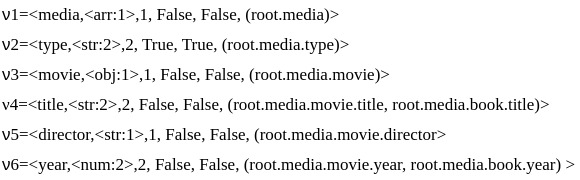
\includegraphics[scale=.43]{Figures/Vertices.jpg}
     \begin{itemize}
         \item \(\nu_1\)=$<$media,$<$arr:1$>$,1, False, False, NULL$>$
         \item \(\nu_2\)=$<$type,$<$str:2$>$,2, True, True, \{cinematography, text\}$>$
         \item \(\nu_3\)=$<$movie,$<$obj:1$>$,1, False, False, NULL$>$
         \item \(\nu_4\)=$<$title,$<$str:2$>$,2, False, False, NULL$>$
         \item \(\nu_5\)=$<$director,$<$str:1$>$,1, False, False, NULL$>$
         \item \(\nu_6\)=$<$year,$<$num:2$>$,2, False, False, NULL$>$
         \item \(\nu_7\)=$<$genres,$<$arr:2$>$,2, True, False, \{fantasy, adventure\}$>$        
     \end{itemize}
\end{example}
Note that the field \textit{type}, for example, appears twice in the collection, and in both cases, it is a string. The same goes for \textit{title} and \textit{year}. 

In the following, we define how a field becomes an enumeration and, if so, a tagged union. 
We use three thresholds to help discovering enumeration and tagged unions: (\textit{i}) \(thr_\Lambda\) to identify whether or not the content of a field may be an enumeration, (\textit{ii})  $Thr_t$ to indicate if the field content is dominated by a given type, and ($iii$) $Thr_{str}$  to check the length of the string in the content of a given field.

\begin{definition} {\it Enumeration}.
 A field from a JSON collection is set as an enumeration (i.e., \textit{isEnum} is true) if and only if  \(\nu \in V\) is associated with a set of values \(\Lambda\) such that: ($i$)  \(\mid\Lambda\mid\) \(\le thr_\Lambda\) and
 %($i$) given $c$ and \(|\Lambda|\), \(\frac{c}{|\Lambda|} \geq Thr_{rat}\),   
 ($ii$) let $t'$   in $\mathcal{T}$ be a tuple with a key:value $t_i$:$occ_i$:
 \begin{itemize}
     \item \(\frac{t'.occ_i}{\sum_{k=1}^{|\mathcal{T}|} t_k.occ_k}\) $\geq Thr_t$;
     \item If $t_i$ is a string type , let $\lambda'$ be the value with the maximum length in $\Lambda$,  $\lambda'$ $\leq$ $Thr_{str}$; and
     %\item If $t_i$ is a numeric type, it must be an integer with maximum of $\Lambda$,  $\lambda'$ $\leq$ $Thr_{int}$.
 \end{itemize}
   \hfill{$\diamond$}
   \label{def:Enum}
\end{definition}

The intuition behind Definition~\ref{def:Enum} is as follows: ($i$) the number of unique values of a given field cannot be greater than a threshold ($Thr_{\Lambda}$), ($ii$) the unique values must have a dominant type ($Thr_t$ $>=$ $n$\% where $n$ is the value), ($iii$) if the predominant type is a string, the length of the larger value cannot be greater than a threshold ($Thr_{str}$), since string enumerate values tend to be small, and ($iv$) float values tend not to compose enumeration values. 
For example, given the set of \textit{genres} values equals to \(\Lambda\)=\{\textit{fantasy, adventure}\},  $Thr_{\Lambda}$ equals 10, $Thr_{t}$ equals 0.8, and $Thr_{str}$ equals 20, \textit{genres} is considered an enumeration.

\begin{definition} {\it Tagged Union}.
A field from a JSON collection is set as a tagged union (i.e., isTU is true) if and only if $\nu \in V$ is an enumeration and its siblings respect the following: ($i$) let \(\lambda_1\) be a distinct value of vertex \(\nu\), so \(\nu.\lambda_1 \rightarrow v' \) are ensured in $G$. 
   \hfill{$\diamond$}
   \label{def:isTU}   
\end{definition}

The relationship \(\alpha \rightarrow \beta\) (\textit{i.e}, a functional dependency) from Definition~\ref{def:isTU} means that $\alpha$ determines the value of $\beta$. 
In our approach, we borrow the functional dependency definition from the database theory to state that, given two vertices \(\nu, \nu' \in V\) and $\lambda_1 \in \Lambda$ in $\nu$, \(\nu.\lambda_1\)  determines a sub-schema $\nu'$.

The following example shows the use of enumeration and tagged union.

\begin{example}
Given the JSON collection from Figure~\ref{fig:JSONEx}, the field \emph{type} is an enumeration since it comprises two distinct values: \emph{cinematography} and \emph{text}. And, it is a tagged union because when its value is cinematography, its right sibling is the field \emph{movie}; otherwise, it is the field \emph{book}. The relationships are \emph{type.cinematography}$\rightarrow$ \emph{movie} and \emph{type.text}$\rightarrow$ \emph{book}. 
On the other hand, the field \emph{genres} is also an enumeration; however, it is not a tagged union. 

\end{example}

\begin{definition} {\it Edge}. 
   An edge \(\varepsilon \in E\) is a tuple \(\varepsilon\)=\(<\)\((\nu_s\), \(\nu_t),\) \(rs, c_\varepsilon\), \(lv_\varepsilon\)\(>\) where (i) (\(\nu_s, \nu_t \in V\)) is a pair representing the source and target of the edge, respectively, (ii) \emph{rs} is the relationship between \(\nu_s\) and  \(\nu_t\) and can assume p or s indicating that \(\nu_s\) is parent or sibling of   \(\nu_t\), respectively, (iii) \(c_\varepsilon\) stores the number of occurrences of \emph{rs} between \(\nu_s\) and  \(\nu_t\), and (iv)  \(lv_\varepsilon\) is a list (possibly empty) that stores the values appearing when \(\nu_t\) is a sibling of \(\nu_s\).
   \hfill{$\diamond$}
   \label{GraphE}
\end{definition}

The components of a tuple in an edge $\varepsilon$ are used as follows: ($i$) \textit{rs} is employed in two flavors: first, to identify the sub-schema of a field when the relationship is $p$ or to determine if \(\nu_s\) is a tagged union candidate, ($ii$) \(c_\varepsilon\) controls whether or not a relationship $rs$ is mandatory (\(\frac{c_{\varepsilon}}{c~in~\nu_s} > Thr_m\)), \textit{i.e.}, the ratio of the number of occurrences of  $\nu_s$ and the number of occurrences of the relationship with  $\nu_t$ is greater than a threshold, and ($iii$) \(lv_\varepsilon\) is used to build a tagged union type.

\begin{example}
    Still using the JSON collection from Figure~\ref{fig:JSONEx}, the following edges belong to the built graph:
    \begin{itemize}
         \item \(\varepsilon_1\)=$<$(book, genres),p,2,NULL$>$
         \item \(\varepsilon_2\)=$<$(movie, director) ,p,1,NULL$>$
         \item \(\varepsilon_3\)=$<$(book, author),p,1,NULL$>$
         \item \(\varepsilon_4\)=$<$(type, book),s,1,(\textquotesingle text\textquotesingle)$>$
         \item \(\varepsilon_5\)=$<$(type, movie),s,1,(\textquotesingle cinematography\textquotesingle)$>$
    \end{itemize}
    
\end{example}

The above definitions state how we build a data structure to represent a JSON collection and use it to extract enumerations and tagged unions. 
Note that we need to set some thresholds (\textit{i.e.}, \(Thr_\Lambda\), \(Thr_t\), \(Thr_{str}\), and \(Thr_m\)) to allow our approach to work correctly. 
We run some experiments to identify the best values for the thresholds. 
In Section \ref{sec:ResDisc}, we present the values used in the main experiments.

Finally, Figure~\ref{fig:graphcoll} shows a graph representation from JSON collection in Figure~\ref{fig:JSONEx}. 
We use ellipses to represent all vertices, except for tagged unions represented by diamonds (field \textit{type}), enumeration by houses (field \textit{genres}), metadata as data by rectangles (vertices \textit{string} and \textit{numeric}), and vertices affected by tagged unions are reached by dotted edges (fields \textit{movie} and \textit{book}). 
Note that, for clarity, not all sibling edges appear in the graph, and we do not show the content of the vertices and edges.

\begin{figure*}[ht]
    \centering
    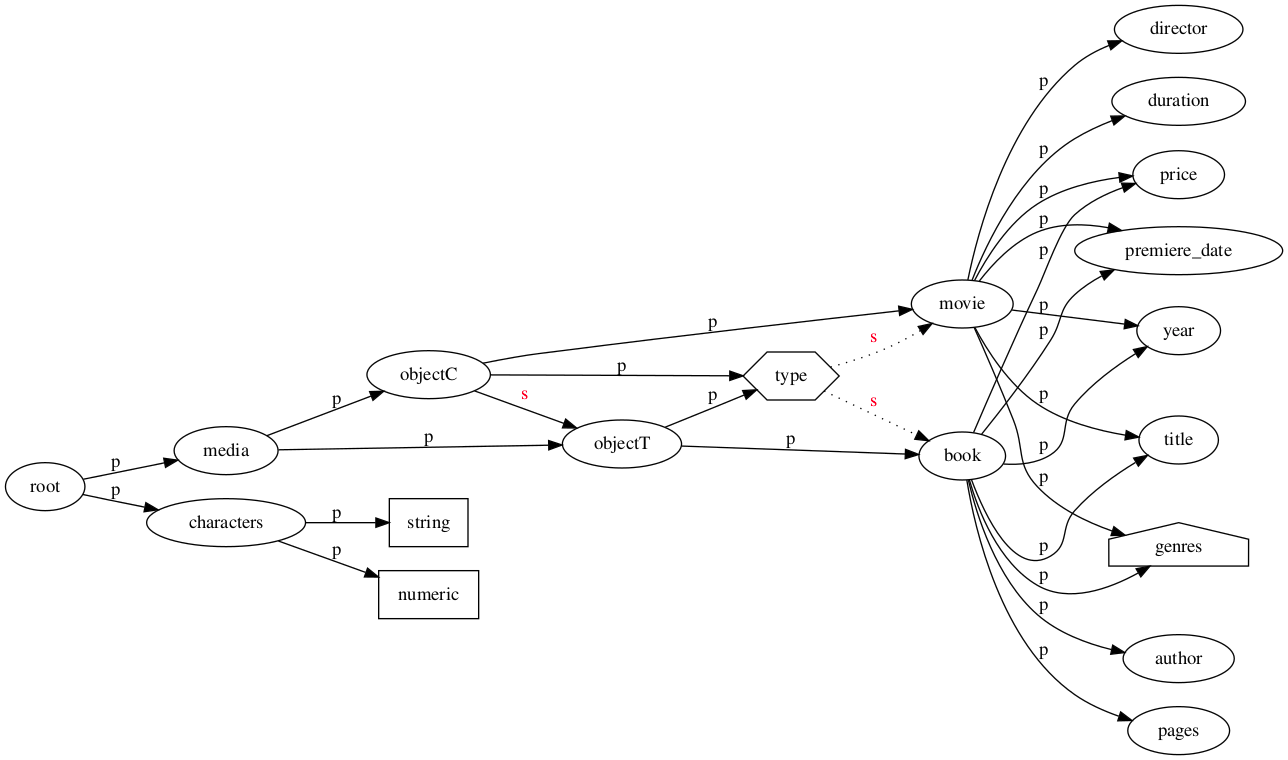
\includegraphics[scale=.35]{Figures/JSONgraph.png}
    \caption{Graph representing the collection in Figure~\ref{fig:JSONEx}.}
    \label{fig:graphcoll}
\end{figure*}

\subsection{Tuples, Collections, and Metadata}

Section~\ref{sec:prelim} shows that it is common sense that array types are composed of collections, and object types are composed of tuples. 
However, some JSON documents do not follow that. If the content of a given array $\mathcal{A}$ is very similar. The similarity is calculated based on the content type and a threshold (see Definition~\ref{def:Thrarr}).  
%(\textit{e.g.}, it contains only numeric atomic types), 
$\mathcal{A}$'s content can be seen as a tuple. 
The same reasoning can be applied to objects: if the content is dissimilar, it represents a collection of other objects. 
Besides, a sub-schema may represent data instead of metadata. 
For example, the content of field \textit{characters} is not a list of \textit{field:value}; it is a list of names with ages, and, in this case, they are not metadata. 
We cannot extract a rule like \textit{characters}: \{``harry potter'': integer ``hermione granger'': integer\} because the characters' names and ages represent data. 
In the following, we formalize some definitions to identify when content is a tuple or a collection. When it is a tuple, the content may be considered data.

\begin{definition}
 \label{def:Thrarr}
    Array as Tuple. Given an array content $\mathcal{C}$, $\mathcal{C}$ is seen as a tuple if and only if ~$\mathcal{C}$ is composed of ~$Thr_{arr}$ of same elements.   \hfill{$\diamond$}
\end{definition}

Note that, from the definition, when the content of an array is very similar, we can consider it as a tuple. 
A threshold is used to take into account noise in the content. 
%Based on our experiments, 90\% (\textit{i.e.}, 0.9) is a reasonable threshold.

\begin{definition}
    Object as Collection. Given an object content $\mathcal{C}$, $\mathcal{C}$ is seen as a collection if and only if ~$\mathcal{C}$ contains ~$Thr_{obj}$ of dissimilar elements.   \hfill{$\diamond$}
\end{definition}

Note that from the definition, when the content of an object contains some dissimilarity, we can consider it as a collection.  
The threshold $Thr_{obj}$ is used to take into account noise in the content. 
%Based on our experiments, over 10\% (\textit{i.e.}, 0.1) is a reasonable threshold.

Finally, we define the problem of data being represented as metadata. This problem was raised in~\citep{Nam21,Sp+21}, and the goal is to find when a JSON sub-schema represents data instead of metadata.

\begin{definition}
    Metadata as data. Given a content \(\mathcal{C}\) of an object seen as a collection, if \(\mathcal{C}\) is composed only of $<$key$>$:$<$value$>$ and more than $Thr_{dt}$\% are optional,  \(\mathcal{C}\) represents data instead of metadata in the collection. 
    \label{def:metadata}
    \hfill{$\diamond$}
\end{definition}

Note that, from Definition~\ref{def:metadata}, the threshold  \(Thr_{dt}\)\% plays an essential role in considering a pair $<$\textit{key}$>$:$<$\textit{value}$>$ as data instead of metadata.  
For example, if a label \textit{L} occurs 50 times, its child \textit{Lc} occurs 48 times, and $Thr_{dt}$\% is set to 95, \textit{Lc} would be mandatory.
 
The content of the field \textit{characters} (Line 23 in Figure~\ref{fig:JSONEx}) is a case of metadata as data: the characters name and age are data. Representing them as metadata, we should use another type of representation, for example, $<$name$>$:\(\mathbb{R}\). 
Instead, the model is \(\mathbb{S}\):\(\mathbb{R}\). 
The optionality of the content leads our approach to consider it as data or metadata. 
%The threshold $Thr_{dt}$ is used for that. %to 70\% to identify whether or not a sub-schema represents data.  

\subsection{JSON Metamodel}
\label{subsec:meta}

We propose a metamodel to represent a conceptual schema for JSON collections. 
Our metamodel is expressed using BNF-like metasyntax (Backus-Naur form). 
BNF is a formal way to describe a language and, in our approach, a JSON schema. 
It consists of a set of terminal and non-terminal symbols. 
The symbols derive a language using production rules in the form \textit{left-hand-side::=right-hand-side}, where LHS (Left-Hand-Side) is a non-terminal symbol, and RHS (Right-Hand-Side) is a sequence of symbols (terminals or non-terminals). 
The meaning of a production rule is the LHS (a non-terminal symbol) may be replaced by the expression represented by RHS.

Accordingly, our meta JSON schema language is defined as follows:
%\setlength{\grammarparsep}{20pt plus 1pt minus 1pt} % increase separation between rules
\setlength{\grammarindent}{81pt} % increase separation between LHS/RHS 
\begin{grammar}
\parsep\grammarparsep
<atm-type> ::= $\mathbb{S}$ | $\mathbb{R}$ | $\mathbb{B}$ | \textit{null}

<field-name> ::= $(\mathbb{S})^+$

<atm-field> ::= <field-name> `:' <at-type>

<arr-type> ::= `[' <arr-value>, $\dots$, <arr-value> `]'

<arr-value> ::= (<atm-type> | <arr-type> | <obj-type>)$^+$

<array> ::= <field-name> `:' <arr-type>

<obj-type> ::= `{' (<atm-field> | <array> | <object>)$^+$ `}'

<object> ::= <field-name> `:' <obj-type>
\end{grammar}

\noindent where ($i$) \(<\)\textit{atm-type}\(>\)  defines the atomic types $\mathbb{S}$, $\mathbb{R}$, $\mathbb{B}$, and  \textit{null} represent a string, numeric, boolean, and null value, respectively and  ($ii$) \(<\)\textit{field-name}\(>\) represents a valid field name in JSON collections. The other constructors follow the same reasoning. 


Finally, enumeration and tagged union production rules can be defined as follows:

\setlength{\grammarindent}{95pt} % increase separation between LHS/RHS 
\begin{grammar}
\parsep\grammarparsep
<enum> ::= <field-name> `:[' <atm-type>, $\dots$, <atm-type> `]'

<tagged-union> ::= `IF' <enum-cond> `THEN' (<atm-field> | <array> | <object>)

<enum-cond> ::= <field-name> `.' <atm-type>
\end{grammar}

The following example shows an instance of our metamodel representing the JSON collection from our running example (Figure~\ref{fig:JSONEx}).

\begin{example}
    ~ \\ \\
    root \hspace{20pt} \textnormal{::=} \{\textbf{media:} arr\_m \textbf{characters:} str\_ch\}\\
    arr\_m \hspace{8pt}  \textnormal{::=}  \textnormal{[}obj\_a\textnormal{]} \\
    obj\_a \hspace{10pt} \textnormal{::=} IF \textbf{type.cinematography} THEN obj\_c \\
    \hspace*{52pt} $\mid$ IF \textbf{type.text} THEN obj\_t \\
    obj\_c \hspace{12pt} \textnormal{::=} \textbf{movie:} obj\_m \\
    obj\_t \hspace{14pt} \textnormal{::=} \textbf{book:} obj\_b \\
    obj\_m \hspace{9pt}  \textnormal{::=} \textbf{title:}$\mathbb{S}$ ~\textbf{director:}$\mathbb{S}$ ~\textbf{year:}$\mathbb{R}$ ~\textbf{premiere\_date}:arr\_date~\textbf{duration:}$\mathbb{R}$ \\
    \hspace*{60pt} \textbf{price:} $\mathbb{N}$ \textbf{genres}:arr\_g \\
    %enum\_g:=\textbf{fantasy} $\mid$ \textbf{adventure} \\
    obj\_b \hspace{11pt} \textnormal{::=} \textbf{title:}$\mathbb{S}$ ~\textbf{author:}$\mathbb{S}$ ~\textbf{year:}$\mathbb{R}$ ~\textbf{premiere\_date}:arr\_date~\textbf{pages:}$\mathbb{R}$ ~\textbf{price:}$\mathbb{R}$ \\
    \hspace*{60pt} \textbf{genres}:~arr\_g\\
    arr\_g \hspace{11pt} \textnormal{::=} \textnormal{[}\textbf{fantasy} , \textbf{adventure}\textnormal{]} \\
    arr\_date \textnormal{::=} \textnormal{[}$\mathbb{R}$, $\mathbb{R}$, $\mathbb{R}$\textnormal{]} \\
    str\_ch \hspace{9pt} \textnormal{::=} \{\textnormal{(}$\mathbb{S}$ \textnormal{:} $\mathbb{R}$\textnormal{)}$^+$\}%\\
\end{example}

Note that \textit{obj\_a} represents a tagged union, \textit{arr\_g} represents an enumeration, \textit{str\_ch} is modeled as pairs \textit{string:string} because the field \textit{characters} is considered a collection and not an object, and \textit{arr\_date} models a tuple encoded in an array representing a date type (MM, DD, YYYY). 
A na\"ive approach would extract \textit{arr\_date} as [$\mathbb{R}(,\mathbb{R})^*$], that is, a sequence of numerical values.
\section{Results and Discussion}
\label{sec:ResDisc}
To demonstrate the quality of JFUSE, we used both real and synthetic JSON collections in our experiments. First, we specified the environment in which the experiments took place, and then, we presented both real and synthetic experiment results.

Based on the definitions mentioned in Section~\ref{sec:SchDisc}, our approach was developed using the C++ programming language. 
It can be found  at \textit{https://github.com/NathyBanhara/JFUSE}. 
The experiments were performed on a server machine with four Intel(R) Xeon(R) CPU E7- 4850 (2.00GHz) and 128 GB RAM, running a Linux 4.15.0-50 kernel (Ubuntu 18.04.2 LTS distribution).  
We ran an empirical experiment on various datasets and studied some JSON collections to find the suitable values for all the thresholds, and they are: 
\(Thr_m \geq 0.9\) , 
\(Thr_t \geq 0.5\), 
\(Thr_{str} \leq 20\), 
%\(Thr_{int} \leq 100\), 
\(Thr_{arr} \geq 0.9\), 
\(Thr_{obj} \leq 0.1\), and 
\(Thr_{dt} \geq 0.7\).


\subsection{Real Data Experiments}
Two JSON document collections were used to test our tool with real data.  
The first one was taken from \citep{Sp+21}. The study case refers to pharmaceutical data (\textit{PHC}), which allows testing on scenarios such as objects as collections and enumeration detection, besides basic types. 
The other one regards Russia's 2018 election tweets user activity (TWC). Obtained from Kaggle\footnote{https://www.kaggle.com/datasets/borisch/russian-election-2018-twitter}, the dataset contains tweet records and it is interesting due to its many optional fields. 
We ran the experiments five times to ensure that there would be no discrepancy in the execution time, and it was verified since the standard deviation was less than 1\%. We reported the execution time average. 

%
As Table~\ref{tab:ComparaReal} shows, with a size of 165Mb and 7,226,980 keys, the pharmaceutical experiments had an average performance time of 1m59.947s. The TWC schema, a much larger collection with 11,5GB and 420,022,871 keys, was generated after about 110m46.484s. 
Regarding the collection size, TWC is 8.7 times bigger than PHC, having 58 times more keys than PHC. 
However, concerning the execution time, TWC was 69 times slower than PHC. 
We believe that the number of keys impacts the computational performance more than the size of collections, and because of that, we believe that our approach scales well when facing huge collections. 
Moreover, the column \textit{Schema Keys} shows the number of keys in the resulting schema: PHC comprises 11 keys and TWC has 210 keys. It shows that the built schemas are concise.

% twitter 8.7 times bigger than pharmaceutic 
% twitter 58 times than pharmaceutic (# of keys)
% Performance 69 times slower than pharmaceutic


\begin{table}[!hbt]
\centering
\small
\caption{Table showing the results obtained from experiments with real data.}
\begin{tabular}{|l|r|r|r|r|}
\hline
\textbf{Collection} & \textbf{Size} & \textbf{Keys} & \textbf{Time (s)} & \textbf{Keys} \\ \hline
Pharmaceutic        & 165Mb         & 7,226,980     & 1m59.947s   & 11      \\ \hline
Twitter             & 11,5GB        & 420,022,871   & 110m46.484s & 210    \\ \hline
\end{tabular}
\label{tab:ComparaReal}
\end{table}

In the following, we present the schema extracted from PHC (based on the meta-model described in Section~\ref{sec:SchDisc}).


\noindent
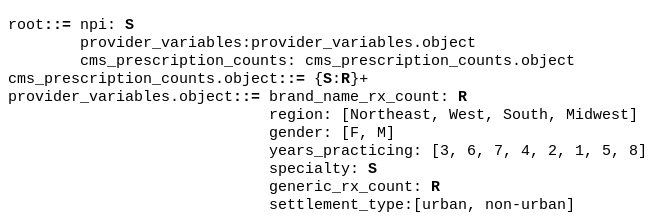
\includegraphics[scale=.6]{Figures/PharmSchema.png}

% \noindent
% \textit{root}::= \textbf{npi:} $\mathbb{S}$ \textbf{provider\_variables:} \textit{provider\_variables.object} \\
% \hspace*{1.2cm} \textbf{cms\_prescription\_counts:} \textit{cms\_prescription\_counts.object}\\
% \textit{cms\_prescription\_counts.object}::= \{($\mathbb{S}$ : $\mathbb{R}$)$^+$\}\\
% \textit{provider\_variables.object}::= \textbf{brand\_name\_rx\_count:} $\mathbb{R}$ \\
% \hspace*{1cm}\textbf{region:} [Northeast, West, South, Midwest] \textbf{gender:} \textit{[F, M]} \\
% \hspace*{1cm}\textbf{years\_practicing:} \textit{[3, 6, 7, 4, 2, 1, 5, 8]} \textbf{specialty:} $\mathbb{S}$ \textbf{generic\_rx\_count:} $\mathbb{R}$ \\
% \hspace*{1cm}\textbf{settlement\_type:} \textit{[urban, non-urban]}

As can be seen, \texttt{cms\_prescription\_counts.object} represents an object as collection, and the metadata inside it is represented as data, which means the optional fields in \texttt{cms\_prescription\_counts.object} are greater than $Thr_{dt}$.  
On the other hand, \texttt{region.string}, \texttt{gender.string}, \texttt{years\_practicing.integer}, and \texttt{settlement\_type.string} are all enumerations.

\subsection{Synthetic Experiments}
We built five new synthetic collections from the Figure~\ref{fig:JSONEx} template to produce collections containing every type that JFUSE intends to discover (\textit{i.e.}, atomic types, tagged unions, metadata, objects as collections, arrays as tuples, and enumeration). 
We ran the experiments five times for the dataset, and we reported the execution time average and the standard deviation. 
Table~\ref{tab:ComparaSyn} shows some statistics from this experiment. %, the results are summarized. Documents with ten thousand, fifty thousand, a hundred thousand, five hundred thousand, and a million objects were targeted. The column Size represents the documents size, whereas Keys, the number of keys in each document. Time is the average time. Deviation shows the deviation in time. 

Note that the execution times follow the number of keys in the collections. 
For example, the third collection contains 2,500K keys, and it took 91.85s to extract the schema; the fourth collection, on the other hand, is 5 times greater than the second one and  took around 4.9 times longer. 
Looking at the standard deviation (\textbf{Std (s)}), we see that all five execution had similar times since the variation is around 2\%. 
Regarding the size of the schemas, our approach is stable, specially when collections follow a pattern (as our synthetic collection does); see column \textbf{Sch Keys} in Table~\ref{tab:ComparaSyn}. 

%Considering the results obtained, it can be inferred both time and schema size scalability.

\begin{table*}[!hbt]
\centering
\small
\caption{Results obtained from experiments with synthetic data.}
\begin{tabular}{|c|c|c|c|c|c|}
\hline
\textbf{Objects} & \textbf{Size (Mb)} & \textbf{Keys} & \textbf{Avg Time (s)} & \textbf{Std (s)} & \textbf{Sch Keys} \\ \hline
10,000           & 12.12              & 250,000       & 8,43              & 0,57   &  11        \\ \hline
50,000           & 60.61              & 1,250,000     & 45,49             & 0,59   &   11       \\ \hline
100,000          & 121.22             & 2,500,000     & 91,85             & 1,18   &   11     \\ \hline
500,000          & 606.09             & 12,500,000    & 452,37            & 7,40   &   11       \\ \hline
1,000,000        & 1,202.19           & 25,000,000    & 922,10            & 19,63  &  11        \\ \hline
\end{tabular}
\label{tab:ComparaSyn}
\end{table*}

\subsection{Final Remarks}

We manually compared the extracted schemas to  samples of the input collections, and we confirmed that   
%Searching the labels extracted from the collection in a sample collection, and comparing their content, 
%our experiments showed that 
JFUSE could extract all the facets it intended to do: enumeration, tagged union, metadata as data, collections, and tuples (see Section~\ref{sec:SchDisc}). 
Moreover, the resulting schemas are concise regarding the size of the input collections, and the execution time is satisfactory. 
We use a synthetic collection to provide a proof of concept for our definitions stated in Section~\ref{sec:SchDisc}. 
The experiments also showed that our approach is scalable. 
Finally, our metamodel can be used as a source to build any JSON schema-language-like.
\section{Conclusion}
\label{sec:Concl}

We introduced a novel approach to extracting schema from JSON collections. The key distinguishing features of our tool are:

\begin{itemize}
    \item Our tool has the unique capability to discover tagged unions, a feature that is not straightforward to extract. This is particularly valuable as a value of an object's property (the tag) conditionally may imply subschemas for sibling properties.
    \item Based on a threshold, field values may be considered as enumeration. It allows the tool to handle variations in data representation, enhancing the accuracy of schema extraction.
    \item Our tool can distinguish between tuples and collections, thereby accurately identifying the content of arrays and objects. This capability significantly improves the reliability of the schema extraction process.
    \item We propose a metamodel that can be transformed into any schema language.
    \item It captures data encoded as metadata, \textit{i.e.}, although a field is encoded as an object, it may represent collections where each element maps keys to values. For example, the field \texttt{characters} from Figure~\ref{fig:JSONEx} is encoded as \textit{character name} and their \textit{age}.
\end{itemize}

Our experiments showed that our approach could extract all the JSON schema facets proposed here, the execution time was satisfactory, and the extracted schema was concise and correct. In future work, we intend to automatize the threshold values, \textit{i.e.}, the tool discovers the best values for a given collection.  

\noindent
\textbf{Acknowledgments}: Natália Banhara was partially funded by Universidade Federal da Fronteria Sul under process number PES-2021-0458.

 

\bibliographystyle{sbc}
\bibliography{refs}

\end{document}
